\documentclass{hbrs-ecta-report}

\usepackage{float}
\usepackage{placeins}
\usepackage{algorithm}
\usepackage{algorithmicx}
\usepackage{algpseudocode}

\begin{document}

\conferenceinfo{H-BRS}{2017}

\title{NeuroEvolution of Augmenting Topologies (NEAT)}
\subtitle{Steuerung eins Mario Jump \& Run Spiels}

\numberofauthors{2}
\author{
Jan Urfei\\
       \affaddr{Bonn-Rhein-Sieg University of Applied Sciences}\\
       \affaddr{Grantham-Allee 20}\\
       \affaddr{53757 Sankt Augustin, Germany}\\
       \email{jan.urfei@inf.h-brs.de}\\
\and
	Tim Lügger\\
	\affaddr{Bonn-Rhein-Sieg University of Applied Sciences}\\
	\affaddr{Grantham-Allee 20}\\
	\affaddr{53757 Sankt Augustin, Germany}\\
	\email{tim.luegger@inf.h-brs.de}\\
}
\date{today}
\maketitle
\begin{abstract}
Ziel war es eine Mario Spielfigur mit bestimmten Szenarien zu trainieren, sodass diese dann das/die Level best möglichst lösen kann.
\end{abstract}

%% ------------------------------ GENERAL NOTES ------------------------------ %%
\section{General Notes}
\label{sec:generalnotes}
\begin{itemize}
\item Do not state things you cannot confirm either by literature or experiment. This is science, not black magic.
\item Normalize your data and resulting statistical descriptors (like RMSE, $\mu$)
\item Save your experimental results to disk \textbf{before you visualize}. You \textbf{will} change your plots quite a lot after gathering the data.
\item Don't submit reports with many pages containing just a single figure. Scrolling is terrible for our health.
\item \textbf{Separate} training and test data. Don't use test data in your algorithm to learn or make decisions, they are only allowed to test the end result. If you need a separate sample set to make decisions during training or optimization, create a third (validation) set. Only your test data will really tell you how good your algorithm is. 
\end{itemize}

\subsection{Algorithm Parametrization}
Develop an actual strategy, preferably on a reduced but similar problem. You can reduce the number of samples, the targetted number of time steps your controller runs in a simulation, or any other non-destructive problem reduction method. If your algorithm has two paramers you need to adjust, it should be no problem to take 5 \textit{sensible} values per parameter and compare all combinations. For stochastic algorithms, like evolutionary approaches, make sure you \textbf{repeat your experiments} at least 5-10 times, depending on the amount of randomness. Since your algorithm makes "random" changes, just comparing single runs does not give you a good estimation on its performance. Do \textbf{not} pick your values such that they only confirm the values you \textbf{want} to use.

%% ------------------------------ STRUCTURE ------------------------------ %%
\subsection{Structure}
\label{sec:structure}
\begin{enumerate}
\item \textbf{Assignment Description}: first provide a brief description of the assignment that was handed out to you. This includes a description of the data.
\item \textbf{Approach}: describe the algorithm
\item \textbf{Experiments}: describe your experimental setup, algorithm parameters, data preprocessing first. Then include the results and a discussion thereof.
\item \textbf{Conclusion}: any conclusions about the algorithm, bugs, future work.
\end{enumerate}
%% ------------------------------ VISUALIZATION ------------------------------ %%
\subsection{Visualization}
\label{sec:visualization}

\begin{itemize}
\item Label your axes
\item Use logarithmic scale when appropriate
\item Use descriptive captions below your figures
\item Add legends if necessary
\item Make fontsizes large enough, linewidths thick enough to be readible in the final report.
\item When making comparisons, make sure the results are either in the \textbf{same} graph or graphs are plotted next to (or close to) each other.
\item \textbf{In short: make sure people can read your figures}
\end{itemize}

%% ------------------------------ REPORT STRUCTURE ------------------------------ %%
\FloatBarrier
\newpage
\newpage
\section{Assignment}
Aufgabe war es den für die HeartRate Prediction implementierten NEAT Algorithmus, der sich an dem Originalpaper \cite{Stanley2002a} orientiert, so zu verändern und anzupassen, dass er ein Problem eines Projektes löst, das sich ausgesucht werden konnte. 

In unserem Fall hieß das, eine Mario Figur durch ein Level zu bringen. Dafür muss eine neue Parametrisierung gefunden werden.

Als Trainingsdaten konnten Level generiert werden, die einen gewünschten Schwierigkeitsgrad besaßen. Die Daten, die man aus dieser Map ziehen konnte, sind die Blöcke zentriert um den Mario herum (siehe Figure \ref{fig:MarioInput}). Dabei ist jedem Blocktyp eine eigene Id zugewiesen. Aufgrund von diesen Daten soll NEAT eine Tastenkombination wählen, um den Mario zu steuern.

\begin{figure}[h!]
	\centering
	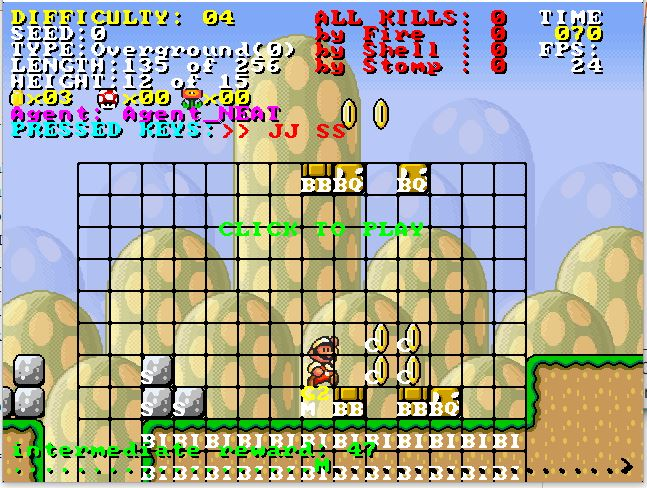
\includegraphics[width=\linewidth]{img/MarioInput.jpg}
	\caption{Umgebungsblöcke des Marios für den Input}
	\label{fig:MarioInput} 
\end{figure}

\FloatBarrier
\section{Approach}

We extend NEAT by including the evolution of the activation function, hoping to produce \textit{leaner} networks that generalize well and take less training\footnote{This would be something you need to show in your results!}. 

\begin{algorithm}[ht!]
\caption{HeteroNEAT}
\label{alg:heteroneat}
\begin{algorithmic}[1]
\State  $c$: $\leftarrow$ mutRate, crossRate, numSpecies, actFcns /* Configuration */
\Statex Input: evalFcn
%\Statex Output:
\Function{HeteroNEAT}{Parameters, Input}
\State $P$: $\leftarrow$ \textbf{\textit{initPop($n$)}} minimal networks
\For{generation $g$}
	\State $N$: $\leftarrow$ expressNetwork($P$)
	\State $F$: $\leftarrow$ evalFcn($N$)
	\State $P$: $\leftarrow$ $(P,N,F)$	/* Assign fitness /*
	\State $S$: $\leftarrow$ speciate($P$,$c$)
	\For{species $s$ in $S$)
		\State $s'(1)$ $\leftarrow$ getElite($s$)
		\State cull($s$,$c$) /* If species is large enough */
		\State $p$: $\leftarrow$ tournamentSelect($s$)
		\State crossover($p$,$c$) /* Combine matching connections */
		\State \textbf{\textit{mutate($p$,$c$)}}
	\EndFor
\EndFor
\EndFunction
\end{algorithmic}
\end{algorithm}

\FloatBarrier
\section{Experiments}
Experiments are repeated 10 times. By the way, this is not enough for a description.

\subsection{Parameterization}
This would include a description of all parameter tuples and a description on how you reduced the problem to provide small and fast runs for this extensive comparison. Results would be shown in boxplots, as these provide you with the median and 25\% and 75\% percentile for every parameter tuple. This makes comparison easy, as you can plot multiple boxplots next to each other, similar as in Figure \ref{fig:4}.

\subsection{NEAT vs ESP}

\begin{figure}[ht!]
\centering
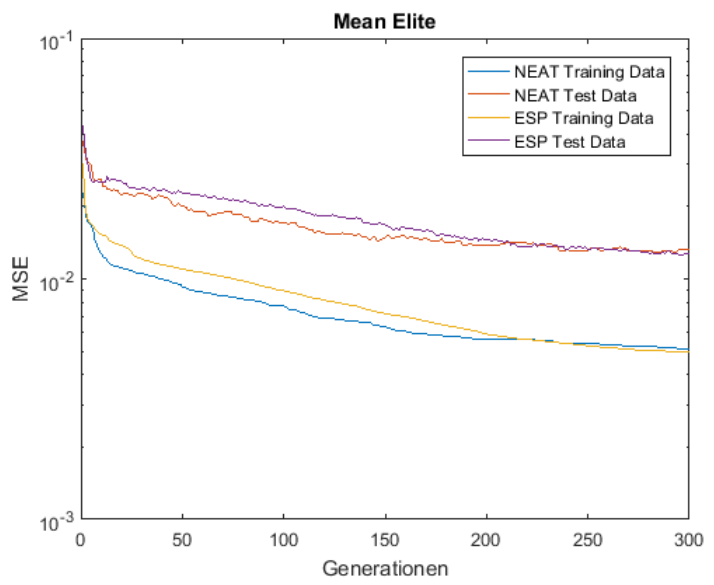
\includegraphics[width=\linewidth]{img/1.png}
\caption{Development of average mean square error, comparing NEAT and ESP}
\label{fig:1} 
\end{figure}
 
\begin{figure}[ht!]
\centering
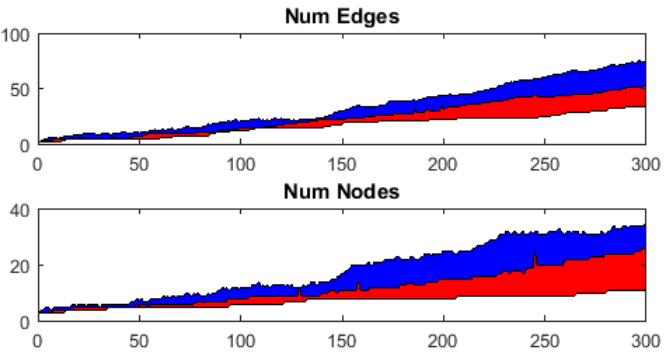
\includegraphics[width=\linewidth]{img/2.png}
\caption{Development of min/mean/max number of nodes and edges. \textit{Legend is missing}!}
\label{fig:2} 
\end{figure}

\begin{figure}[ht!]
\centering
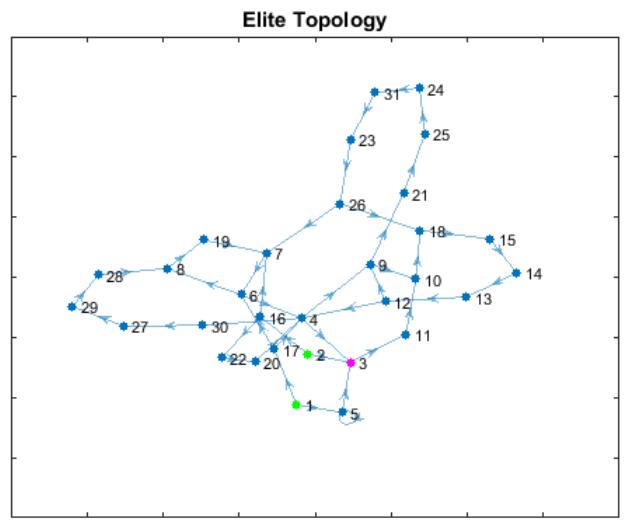
\includegraphics[width=\linewidth]{img/3.png}
\caption{Elite topology. Nodes are assigned their IDs. Green are input nodes, purple are output nodes.}
\label{fig:3} 
\end{figure}

\begin{figure}[ht!]
\centering
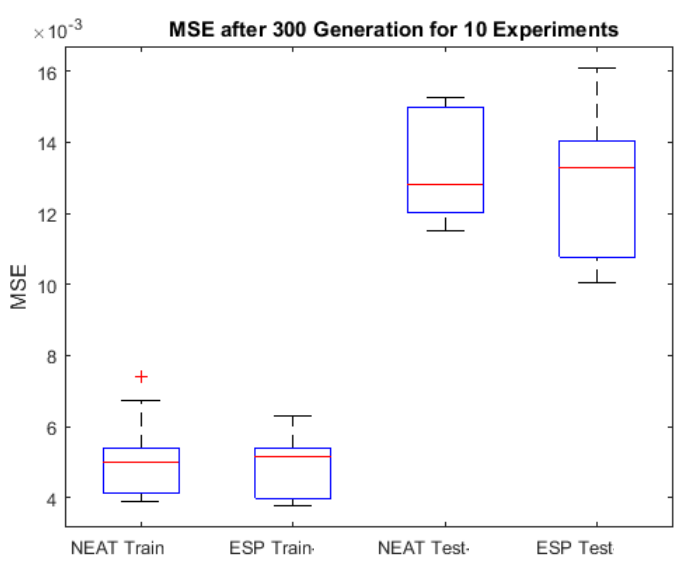
\includegraphics[width=\linewidth]{img/4.png}
\caption{Comparing MSE of NEAT and ESP}
\label{fig:4} 
\end{figure}

\begin{figure}[ht!]
\centering
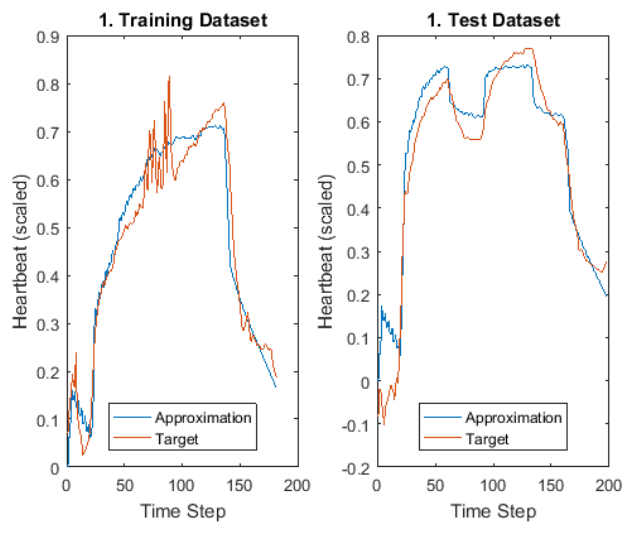
\includegraphics[width=\linewidth]{img/5.png}
\caption{Approximated heart rates after 300 generations}
\label{fig:5} 
\end{figure}

\begin{figure}[ht!]
\centering
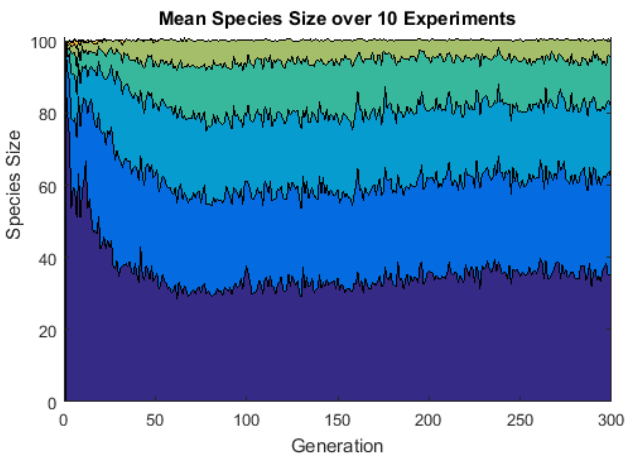
\includegraphics[width=\linewidth]{img/6.png}
\caption{Development of species over time, averaged over 10 generations}
\label{fig:6} 
\end{figure}


\FloatBarrier
\section{Conclusion}


\bibliographystyle{abbrv}
\bibliography{HeteroNEAT} 
\end{document}
}